\chapter{压强、自由能与能量涨落}

\lectureoverview{我们不假设分子撞击器壁的动理学图像，而是从配分函数导出压强。一个几何引理把绝热导数化为固定温度下的导数，亥姆霍兹自由能提供了通向\(\log Z\)的桥梁，理想气体定律则作为第一个应用随之得出。随后我们用同一个配分函数导出平衡能量涨落及其与热容的关系。}

\section{让数学来检验直觉}

热力学有着一种奇特的名声。它的微积分是初等的，然而选择对什么求导、把什么固定住却可能极为微妙。我们的问题是有意收窄的：计算理想气体的压强。然而，通往这一答案的路径被设计得足够普遍，以便适用于那些熟悉的分子图像不再可靠的情形。

动理学的说法很容易讲。分子撞击器壁，并使其动量的法向分量反向。单位时间内传递的动量给出力，而单位面积上的力给出压强。我们已经知道，三维中每个分子的平均动能为
\begin{equation}
 \left\langle \frac{p^2}{2m}\right\rangle=\frac{3}{2}T
 \qquad (k_B=1).
 \label{eq:sm5-mean-kinetic-energy}
\end{equation}
在速度分布各向同性的情况下，人们可以估计碰撞率、每次碰撞中的动量转移以及由此产生的压强。

但器壁本身似乎破坏了各向同性。为什么紧邻边界的分子应当与内部深处的分子具有相同的速率和方向分布？在平衡态下，就此处相关的精度而言，它们确实如此，但这一结论应当从统计力学得出，而不是作为直觉偷偷塞进计算之中。分子之间的碰撞使动理论论证更加不透明。无相互作用气体之所以容易，恰恰因为它是一个异常简单的系统。

物理学中有些时候，最稳妥的做法是暂时压制图像，让数学来驾驭。人们先确定待求的量，操纵一般关系，然后等待一个可辨认的公式出现。直觉在最后回归，但那时是数学在检验直觉，而不是反过来。热力学的乐趣就在于这一过程中涌现出的令人惊讶的关系。

所需的关系是一个状态方程，
\begin{equation}
 P=P(T,V,N),
 \label{eq:sm5-equation-of-state-target}
\end{equation}
其中\(N\)是物质的量，\(T\)是温度，\(V\)是体积。一个令人满意的推导应当在粒子相互作用时，或者当物质是液体、等离子体或固体时，仍然说得通。只有配分函数的最终求值才会专门化到理想气体。

\section{熵与亥姆霍兹自由能}

首先取回后面将要用到的正则公式。对于以\(i\)标记的微观态，
\begin{equation}
 \begin{aligned}
 S&=-\sum_i p_i\log p_i,\\
 p_i&=\frac{e^{-\beta E_i}}{Z},\\
 Z&=\sum_i e^{-\beta E_i}.
 \end{aligned}
 \label{eq:sm5-canonical-definitions}
\end{equation}
概率的对数为
\begin{equation}
 \log p_i=-\beta E_i-\log Z.
 \label{eq:sm5-log-probability}
\end{equation}
代入熵的表达式得到
\begin{align}
 S
 &=-\sum_i p_i\log p_i \notag\\
 &=\beta\sum_i p_iE_i+\log Z\sum_i p_i \notag\\
 &=\beta E+\log Z.
 \label{eq:sm5-entropy-log-z}
\end{align}
这里\(E=\sum_i p_iE_i\)是平均能量。

\begin{classroomqa}
\audiencequestion{为什么第二项只给出\(\log Z\)，而不是态数乘以\(\log Z\)？}
\lecturerresponse{被求和的系数是\(p_i\)，而不是\(1\)。归一化给出\(\sum_i p_i=1\)。等价地，分子\(\sum_i e^{-\beta E_i}=Z\)与分母中的\(Z\)相消。态数在这一步中从未出现。
\lecturetimestamp{00:14:25--00:14:55}}
\end{classroomqa}

在本讲大部分内容所用的能量单位下，
\(\beta=1/T\)。将\eqref{eq:sm5-entropy-log-z}乘以\(T\)并重新整理，得到
\begin{equation}
 E-TS=-T\log Z.
 \label{eq:sm5-helmholtz-identity}
\end{equation}
左边的组合出现得如此频繁，值得给它一个名字：
\begin{equation}
 A\equiv E-TS,
 \qquad
 A=-T\log Z.
 \label{eq:sm5-helmholtz-definition}
\end{equation}
它就是亥姆霍兹自由能。此刻这个名字不如这个恒等式本身重要；当把压强转化为配分函数的导数时，我们将需要这个恒等式。

\begin{figure}[t]
\centering
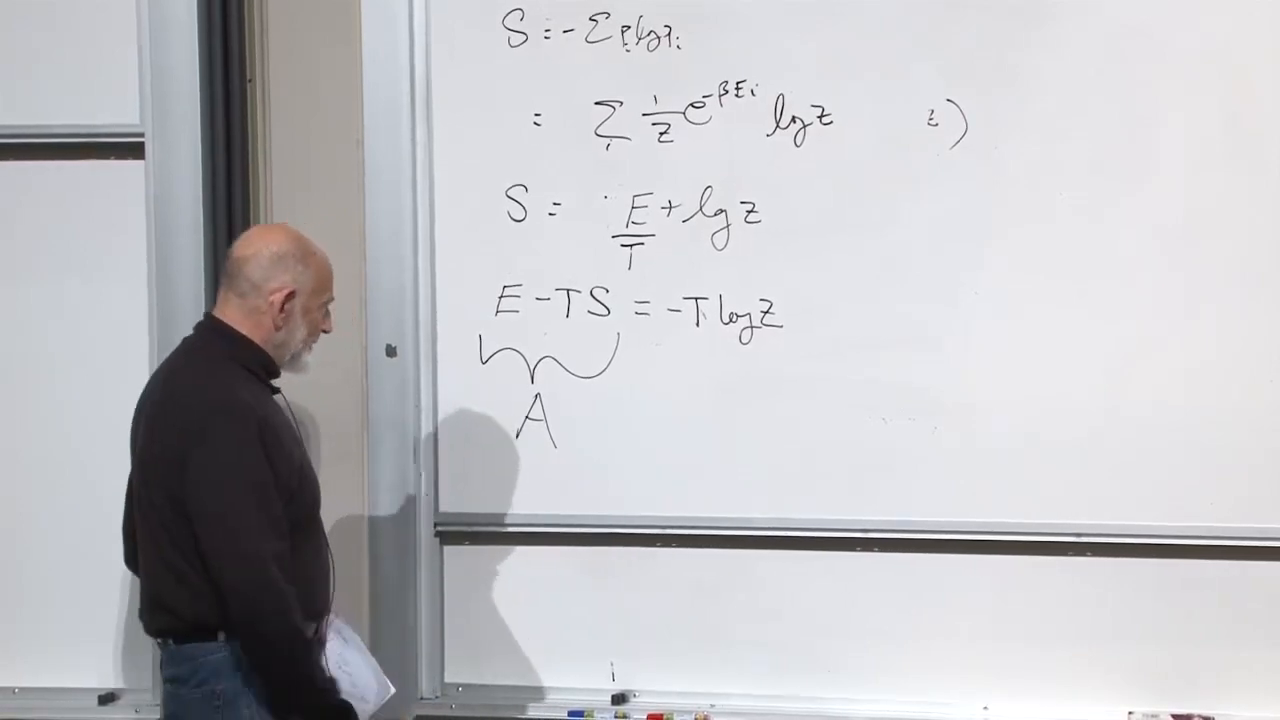
\includegraphics[width=0.90\textwidth]{lecture_05_figure_03.png}
\caption{正则熵关系被重新整理为
\(A=E-TS=-T\log Z\)。}
\lectureframe{00:16:50}
\end{figure}

\section{控制参量及其响应}

控制参量是实验者可以从外部改变的宏观量。移动活塞改变体积，而无需操纵单个分子。外加电场和磁场是另外的例子。在更一般的系综中，粒子数也可以被允许改变。

热力学变量自然地成共轭对出现。体积是当前问题中的控制参量，压强是它的响应。我们改变\(V\)；压强告诉我们系统在能量上如何抵抗这一改变。稍后，能量的导数将使这种配对变得精确。

\begin{classroomqa}
\audiencequestion{压力本身能否被视为控制参量？}
\lecturerresponse{人们可以设计一个固定外部压力的实验，但在本文所用的构造中，活塞位置固定体积，而内部压力是响应量。压力与体积是共轭变量；其中哪一个被控制取决于系综和装置。
\lecturetimestamp{00:19:22--00:20:01}}
\end{classroomqa}

\begin{classroomqa}
\audiencequestion{是否假定所有分子都相同，还是该论证仅限于气体？}
\lecturerresponse{热力学论证不需要这样的限制。圆筒中可以含有多种组分、液体，甚至正在被压缩的固体。只有在一般压力公式建立之后，理想气体配分函数才会成为一个特殊应用。
\lecturetimestamp{00:20:02--00:20:39}}
\end{classroomqa}

\begin{classroomqa}
\audiencequestion{物质的量能否作为另一种外部操作而改变？}
\lecturerresponse{可以。粒子数也是一种可能的控制参量。对它作动力学处理会引出其自身的共轭变量，即化学势。对于今晚的计算，\(N\)保持固定。
\lecturetimestamp{00:20:39--00:20:57}}
\end{classroomqa}

\begin{classroomqa}
\audiencequestion{液态水和蒸汽能否同时处于平衡？}
\lecturerresponse{在共存温度和压力下，它们可以。重力可能使液体位于蒸气下方，但两相仍可共享同一温度并保持热平衡。同一套一般统计力学框架仍然适用。
\lecturetimestamp{00:20:59--00:21:36}}
\end{classroomqa}

对于接下来的论证，把能量和熵视为两个可独立调节变量的依赖函数：
\begin{equation}
 E=E(T,V),
 \qquad
 S=S(T,V).
 \label{eq:sm5-dependent-functions}
\end{equation}
温度和体积给出热力学状态空间上的坐标。能量和熵为该空间中的每一个平衡点赋予数值。

\section{定熵导数}

我们最终需要的导数并不寻常：
\[
 \left(\frac{\partial E}{\partial V}\right)_S.
\]
尽管\(T\)和\(V\)是独立坐标，这个导数要求我们在约束依赖函数\(S(T,V)\)保持恒定的同时改变\(V\)。它是沿\((T,V)\)平面中一条曲线的导数，而不是沿坐标轴的导数。

\begin{classroomqa}
\audiencequestion{如果后面要用到导数\(dT/dV\)，那么\(T\)和\(V\)怎么还能是独立的？}
\lecturerresponse{在整个状态空间上，它们是独立的。一旦施加约束\(S(T,V)=\mathrm{constant}\)，允许的状态就位于一条一维等值线上。沿该等值线，\(T\)成为\(V\)的函数，其斜率\(dT/dV\)有良好定义。
\lecturetimestamp{01:01:18--01:02:09}}
\end{classroomqa}

\begin{lemma}
若\(E(T,V)\)和\(S(T,V)\)可微，则在\((\partial S/\partial T)_V\neq0\)处，
\begin{equation}
 \left(\frac{\partial E}{\partial V}\right)_S
 =
 \left(\frac{\partial E}{\partial V}\right)_T
 -
 \left(\frac{\partial E}{\partial S}\right)_V
 \left(\frac{\partial S}{\partial V}\right)_T.
 \label{eq:sm5-calculus-lemma}
\end{equation}
\end{lemma}

\begin{proof}
对于任意无穷小位移，
\begin{equation}
 dE=
 \left(\frac{\partial E}{\partial V}\right)_T dV
 +
 \left(\frac{\partial E}{\partial T}\right)_V dT.
 \label{eq:sm5-total-differential-e}
\end{equation}
在固定\(V\)时，链式法则允许把\(S\)用作中间变量：
\begin{equation}
 \left(\frac{\partial E}{\partial T}\right)_V
 =
 \left(\frac{\partial E}{\partial S}\right)_V
 \left(\frac{\partial S}{\partial T}\right)_V.
 \label{eq:sm5-chain-rule-e-s-t}
\end{equation}

现在把位移限制在\(S\)为常数的等值线上。沿该等值线，
\begin{equation}
 0=dS=
 \left(\frac{\partial S}{\partial V}\right)_T dV
 +
 \left(\frac{\partial S}{\partial T}\right)_V dT.
 \label{eq:sm5-constant-entropy-differential}
\end{equation}
解出等值线斜率，得到
\begin{equation}
 \left(\frac{dT}{dV}\right)_S
 =
 -
 \frac{\left(\frac{\partial S}{\partial V}\right)_T}
 {\left(\frac{\partial S}{\partial T}\right)_V}.
 \label{eq:sm5-entropy-contour-slope}
\end{equation}
用\(dV\)除\eqref{eq:sm5-total-differential-e}，使用
\eqref{eq:sm5-chain-rule-e-s-t}，并代入
\eqref{eq:sm5-entropy-contour-slope}：
\begin{align}
 \left(\frac{\partial E}{\partial V}\right)_S
 &=
 \left(\frac{\partial E}{\partial V}\right)_T
 +
 \left(\frac{\partial E}{\partial S}\right)_V
 \left(\frac{\partial S}{\partial T}\right)_V
 \left(\frac{dT}{dV}\right)_S \notag\\
 &=
 \left(\frac{\partial E}{\partial V}\right)_T
 -
 \left(\frac{\partial E}{\partial S}\right)_V
 \left(\frac{\partial S}{\partial V}\right)_T.
\end{align}
因子\((\partial S/\partial T)_V\)已经消去，从而证明了该结果。
\end{proof}

\begin{figure}[t]
\centering
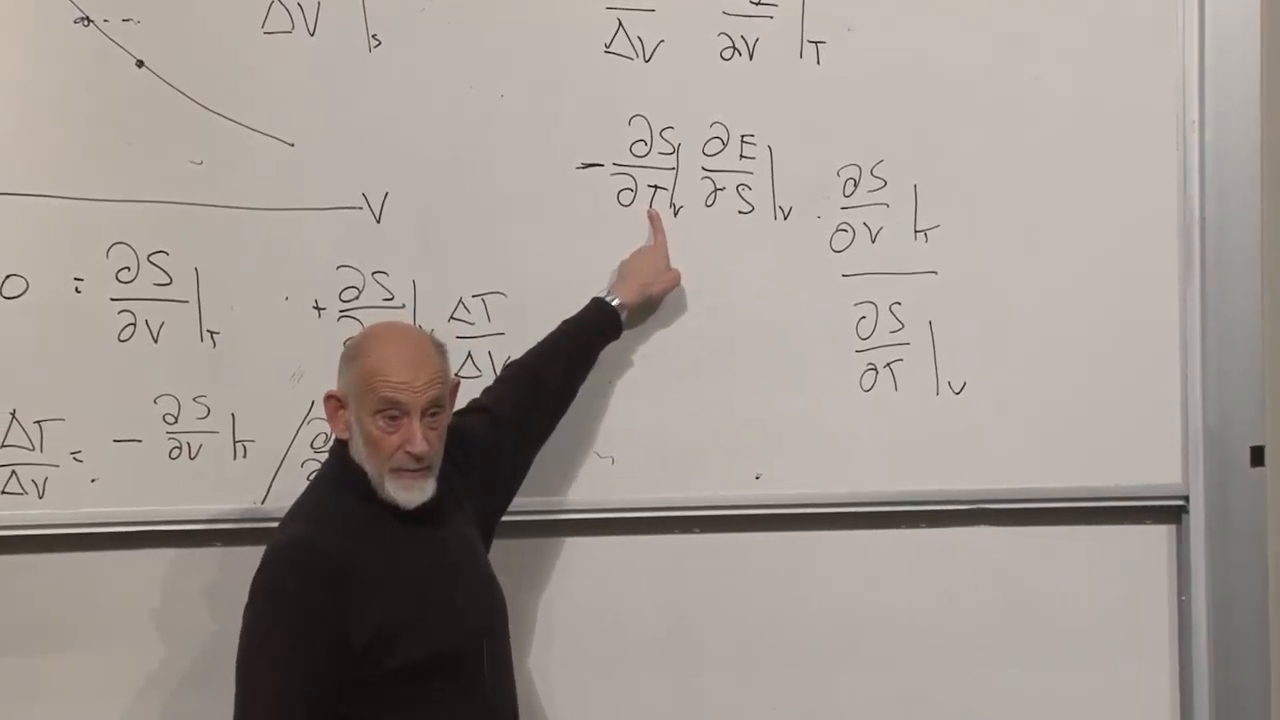
\includegraphics[width=0.90\textwidth]{lecture_05_figure_04.png}
\caption{完成导数引理的定熵等值线计算中的消去。}
\lectureframe{00:36:10}
\end{figure}

几何图像并非装饰。它解释了为什么一个看似奇怪的固定\(S\)导数可以用独立坐标\(T\)和\(V\)下的普通偏导数来求值。在构造过程中写出\(\delta E/\delta V\)，有助于提醒我们这些符号表示沿指定路径的小变化之比。

\begin{classroomqa}
\audiencequestion{\(dE\)的展开是否只是偏导数的普通定义？}
\lecturerresponse{是的。全微分中没有任何特殊之处。唯一额外的要素是随后限制到等值线\(dS=0\)，这决定了\(dT\)与\(dV\)之间的关系。
\lecturetimestamp{00:29:26--00:29:32}}
\end{classroomqa}

\begin{classroomqa}
\audiencequestion{消去是否要求\((\partial S/\partial T)_V\)非零？}
\lecturerresponse{是的。对于普通稳定系统，
\[
 \left(\frac{\partial S}{\partial T}\right)_V
 =\frac{C_V}{T}>0,
\]
所以该除法是合法的。例外点需要另行处理。在哈密顿量固定时，升高温度会加宽正则能量分布，通常增大熵；降低温度则使其变窄。这就是单调性论证在物理上正确的方向。
\lecturetimestamp{00:36:50--00:37:47}}
\end{classroomqa}

\section{活塞功与绝热条件}

现在我们来赋予这个导数物理意义。考虑一个横截面积为\(\mathcal A\)的活塞。如果它向外移动\(dx\)，那么
\begin{equation}
 dV=\mathcal A\,dx.
 \label{eq:sm5-piston-volume}
\end{equation}
气体对活塞施加力\(P\mathcal A\)，因此气体所做的功为
\begin{equation}
 \delta W_{\mathrm{by}}=P\mathcal A\,dx=P\,dV.
 \label{eq:sm5-piston-work}
\end{equation}
如果没有热量进入气体，能量守恒给出
\begin{equation}
 dE=-P\,dV.
 \label{eq:sm5-adiabatic-work}
\end{equation}
符号具有物理意义：在膨胀过程中，气体提升或加速活塞，而自身的能量减少。

\begin{figure}[t]
\centering
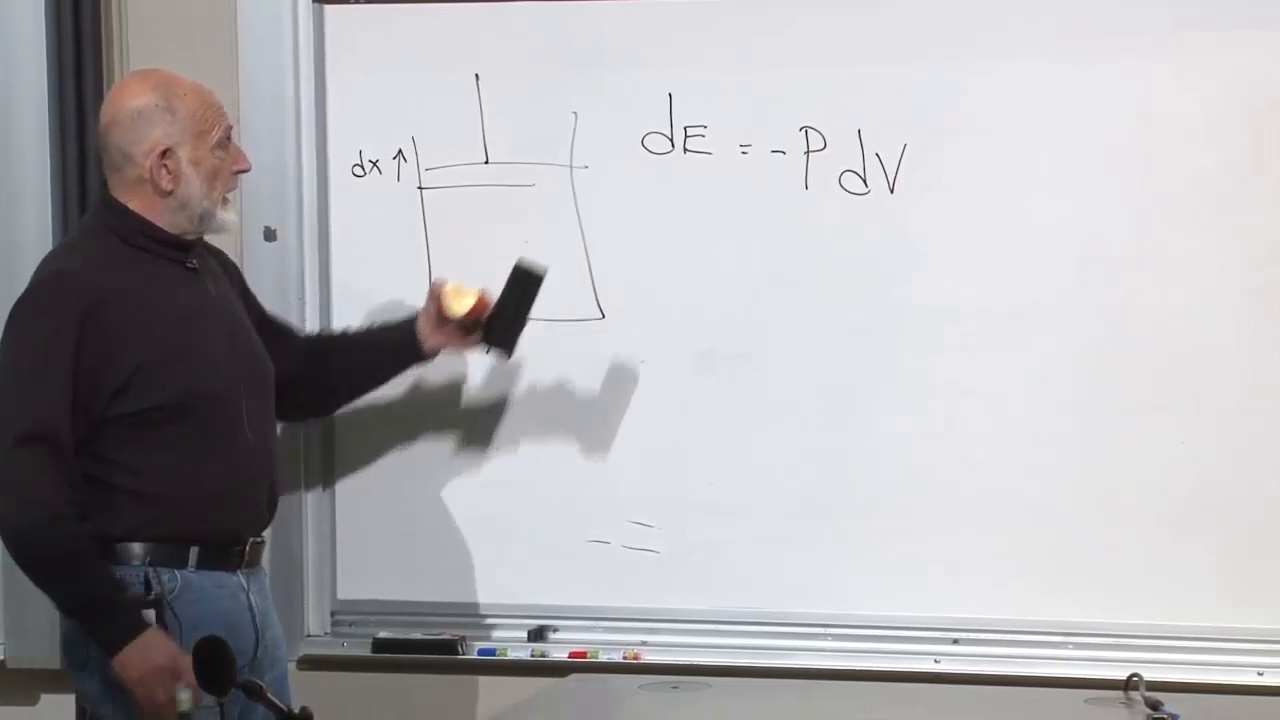
\includegraphics[width=0.90\textwidth]{lecture_05_figure_05.png}
\caption{活塞几何与已完成的功关系\(dE=-P\,dV\)。}
\lectureframe{00:43:10}
\end{figure}

两个限定条件至关重要。活塞必须移动得足够慢，使系统始终任意接近平衡态，并且器壁必须绝热，使能量不以热的形式供给。快速拉动可能快到在运动过程中没有任何分子能够追上后退的活塞。快速压缩会激发冲击波。这两种过程都不能用一系列平衡态来表示。

\emph{绝热}一词有时用于表示无热传递，有时用于表示缓慢变化。在此处所需的可逆过程中，两种含义都涉及：变化是准静态的且热绝缘的。在这些条件下，它也是等熵的。

\begin{classroomqa}
\audiencequestion{为什么绝热变化保持熵不变？}
\lecturerresponse{从量子力学角度考察系统。其多体能级依赖于体积。当\(V\)缓慢变化时，绝热定理将每个被占据的能级连续地变为其后继能级，而不发生能级标号之间的跃迁。能量\(E_i(V)\)发生移动，但占据概率\(p_i\)保持不变。由于
\(S=-\sum_i p_i\log p_i\)依赖于这些概率，熵保持不变。热交换或不可逆运动会使这一结论失效。
\lecturetimestamp{00:43:37--00:49:15}}
\end{classroomqa}

\begin{figure}[t]
\centering
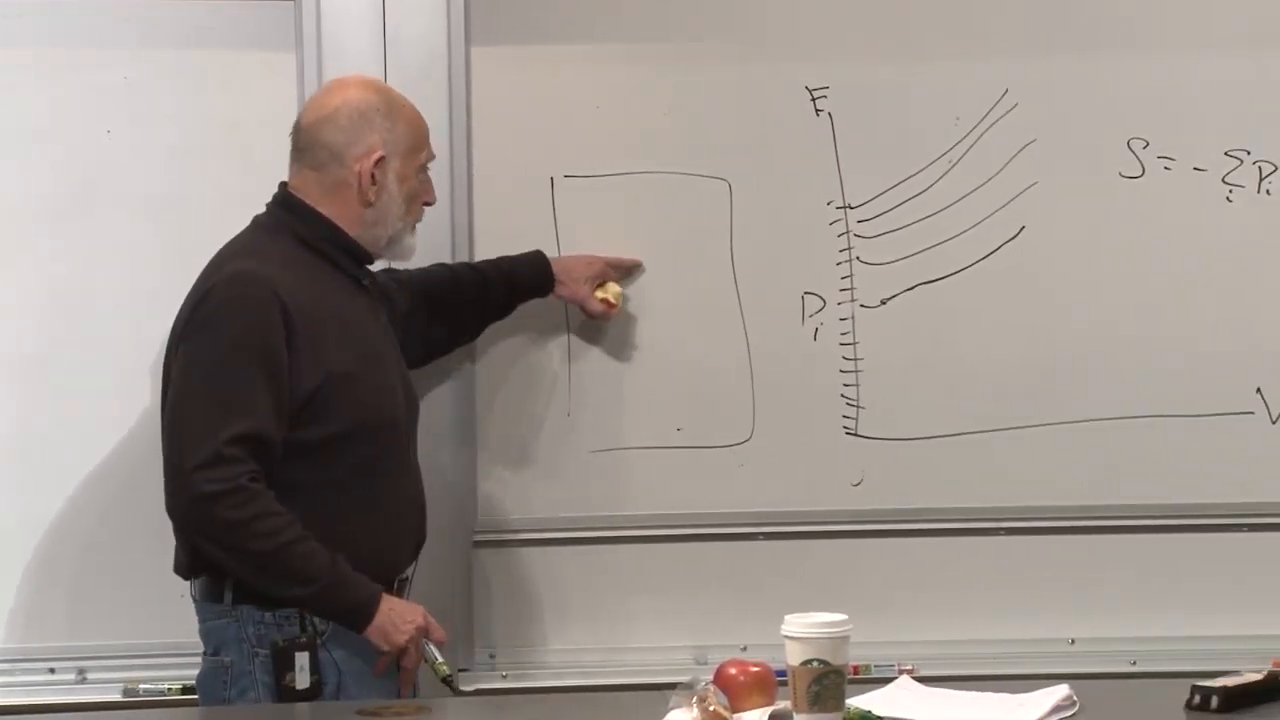
\includegraphics[width=0.90\textwidth]{lecture_05_figure_06.png}
\caption{多体能级随体积移动，而其占据概率保持其能级标号。}
\lectureframe{00:48:50}
\end{figure}

方程\eqref{eq:sm5-adiabatic-work}沿这条等熵路径求值，将压强确定为
\begin{equation}
 P=-\left(\frac{\partial E}{\partial V}\right)_S.
 \label{eq:sm5-pressure-fixed-entropy}
\end{equation}
这就是压强与体积之间的共轭关系。

\begin{classroomqa}
\audiencequestion{如果改为快速移动活塞会发生什么？}
\lecturerresponse{系统离开平衡态，其详细动力学变得重要。突然压缩会产生冲击波。在理想的自由膨胀中，活塞可以在任何分子撞击它之前后退，因此不做功，即使体积发生变化，能量也保持不变。气体随后弛豫到具有增加熵的平衡态。这类过程不能用
\eqref{eq:sm5-pressure-fixed-entropy}中的单一平衡导数来描述。
\lecturetimestamp{00:58:30--01:01:15}}
\end{classroomqa}

\begin{classroomqa}
\audiencequestion{什么定量条件决定一个变化是否缓慢？}
\lecturerresponse{外部变化时间必须远长于相关的内部弛豫时间。对于气体，在宏观变化期间应发生许多分子碰撞和许多器壁撞击。精确的时间尺度取决于材料和几何形状，而准静态极限本身是普遍的。
\lecturetimestamp{01:02:09--01:03:20}}
\end{classroomqa}

\section{从绝热能量到配分函数}

物理公式\eqref{eq:sm5-pressure-fixed-entropy}还不是容易计算的形式。正则系综统计力学自然地给出温度的函数，因为\(T\)直接出现在玻尔兹曼权重中。微积分引理将难以处理的固定熵导数转化为那种计算语言：
\begin{align}
 P
 &=
 -\left(\frac{\partial E}{\partial V}\right)_T
 +
 \left(\frac{\partial E}{\partial S}\right)_V
 \left(\frac{\partial S}{\partial V}\right)_T.
 \label{eq:sm5-pressure-lemma-substitution}
\end{align}
在固定体积下，第一定律给出\(dE=T\,dS\)，因此
\begin{equation}
 \left(\frac{\partial E}{\partial S}\right)_V=T.
 \label{eq:sm5-e-s-temperature}
\end{equation}
于是
\begin{equation}
 P=
 -\left(\frac{\partial E}{\partial V}\right)_T
 +
 T\left(\frac{\partial S}{\partial V}\right)_T.
 \label{eq:sm5-pressure-fixed-temperature-pieces}
\end{equation}

\begin{classroomqa}
\audiencequestion{压强公式中的负号从何而来？}
\lecturerresponse{它起源于气体所做的功：
\(dE=-P\,dV\)在绝热膨胀过程中。微积分引理本身在其两项之间有一个负号；
\(P=-(\partial E/\partial V)_S\)中的整体负号将两者都反转，产生
\eqref{eq:sm5-pressure-fixed-temperature-pieces}。
\lecturetimestamp{00:52:40--00:53:14}}
\end{classroomqa}

由于\(T\)在两个导数中都保持固定，
\begin{align}
 P
 &=
 -\left(\frac{\partial}{\partial V}(E-TS)\right)_T \notag\\
 &=
 -\left(\frac{\partial A}{\partial V}\right)_T.
 \label{eq:sm5-pressure-free-energy}
\end{align}
最后代入\(A=-T\log Z\)：
\begin{equation}
 \boxed{
 P=
 T\left(\frac{\partial\log Z}{\partial V}\right)_T
 }.
 \label{eq:sm5-pressure-log-z}
\end{equation}

\begin{figure}[t]
\centering
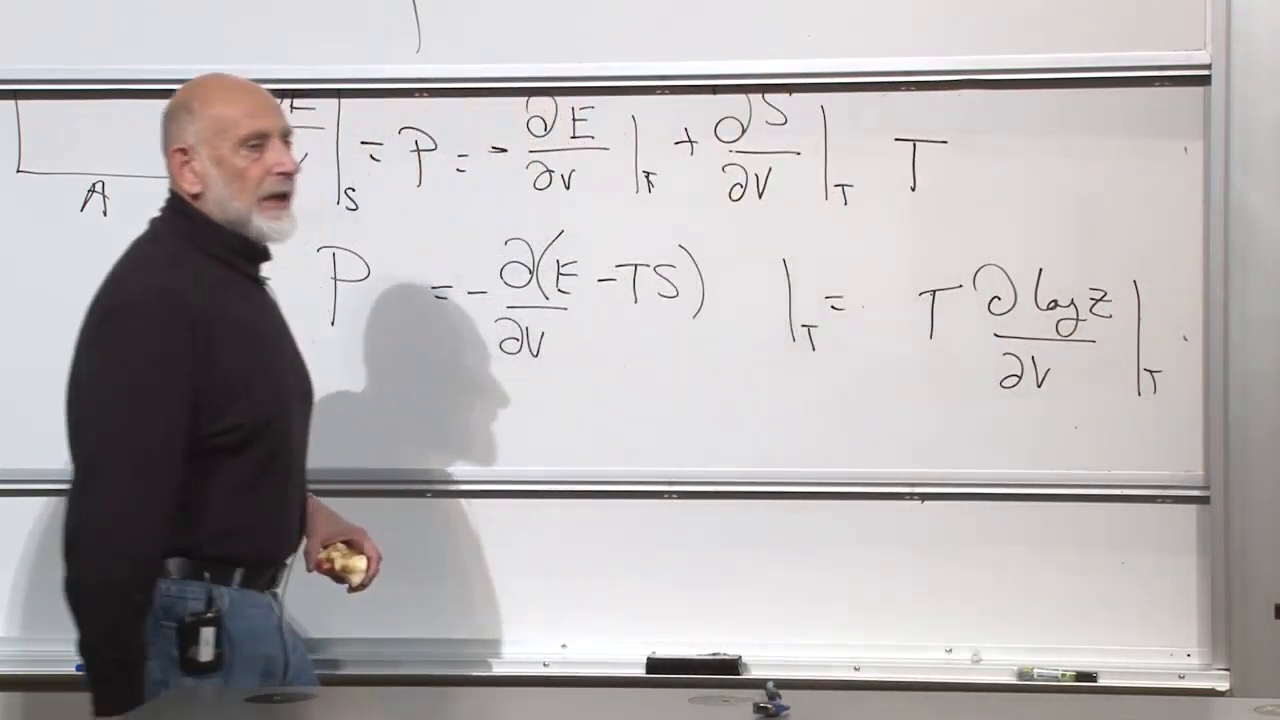
\includegraphics[width=0.90\textwidth]{lecture_05_figure_07.png}
\caption{对宗量的固定温度压缩：
\(P=-(\partial A/\partial V)_T
=T(\partial\log Z/\partial V)_T\)。}
\lectureframe{00:55:55}
\end{figure}

\eqref{eq:sm5-pressure-log-z}中没有任何内容假设理想气体。如果能够为相互作用的流体、等离子体或固体计算出配分函数，同一个导数就给出其压强。更一般地，每个外部控制参数都有一个共轭响应，通过对适当的热力学势求导得到。配分函数将许多这样的响应打包在一起：对\(\log Z\)关于\(\beta\)求导给出能量，而对其关于体积求导给出压强。

\section{理想气体状态方程}

现在才专门考虑\(N\)个无相互作用粒子。保留经典相空间归一化，
\begin{equation}
 Z_N=
 \frac{1}{N!h^{3N}}
 \int d^{3N}q\,d^{3N}p\,
 \exp\!\left[
 -\beta\sum_{a=1}^{N}\frac{\mathbf p_a^2}{2m}
 \right].
 \label{eq:sm5-ideal-gas-partition-integral}
\end{equation}
这里有\(3N\)个位置坐标和\(3N\)个动量坐标。哈密顿量不依赖于位置，因此每个粒子贡献一个容器体积因子：
\begin{equation}
 Z_N=
 \frac{V^N}{N!h^{3N}}I_p(\beta),
 \label{eq:sm5-ideal-gas-factorization}
\end{equation}
其中整个动量积分\(I_p(\beta)\)与\(V\)无关。

\begin{classroomqa}
\audiencequestion{为什么有\(3N\)个位置积分和\(3N\)个动量积分？}
\lecturerresponse{\(N\)个粒子中的每一个都有三个空间坐标和三个共轭动量分量。相空间每一半中的计数都是\(3N\)，而不是\(N\)个粒子加上另外\(3N\)个粒子。
\lecturetimestamp{01:04:19--01:04:28}}
\end{classroomqa}

取对数将体积依赖性分离出来：
\begin{equation}
 \log Z_N
 =
 N\log V-\log N!-3N\log h+\log I_p(\beta).
 \label{eq:sm5-log-ideal-gas-partition}
\end{equation}
因子\(1/N!\)、\(h^{-3N}\)和\(I_p(\beta)\)都与体积无关。它们对绝对熵和其他问题有影响，但对这个特定的导数没有影响。因此
\begin{equation}
 \left(\frac{\partial\log Z_N}{\partial V}\right)_T
 =\frac{N}{V}.
 \label{eq:sm5-log-z-volume-derivative}
\end{equation}
方程\eqref{eq:sm5-pressure-log-z}立即给出
\begin{equation}
 P=\frac{NT}{V},
 \qquad
 \boxed{PV=NT}.
 \label{eq:sm5-ideal-gas-law}
\end{equation}

\begin{classroomqa}
\audiencequestion{\(N\)是否仍然计入用于推导玻尔兹曼分布的复制品？}
\lecturerresponse{不。复制品构造是先前推导中的一种计数手段，现在已不再存在。这里\(N\)是这一个气体样本中的物理粒子数。
\lecturetimestamp{01:07:38--01:08:05}}
\end{classroomqa}

定义数密度
\begin{equation}
 \rho=\frac{N}{V}
 \label{eq:sm5-number-density}
\end{equation}
得到等价形式
\begin{equation}
 P=\rho T.
 \label{eq:sm5-density-equation-of-state}
\end{equation}

\begin{classroomqa}
\audiencequestion{密度形式应该通过除以\(N\)还是除以\(V\)来得到？}
\lecturerresponse{将\(PV=NT\)除以\(V\)：
\(P=(N/V)T=\rho T\)。这里\(\rho\)是数密度，不是质量密度。
\lecturetimestamp{01:08:45--01:09:16}}
\end{classroomqa}

\begin{figure}[t]
\centering
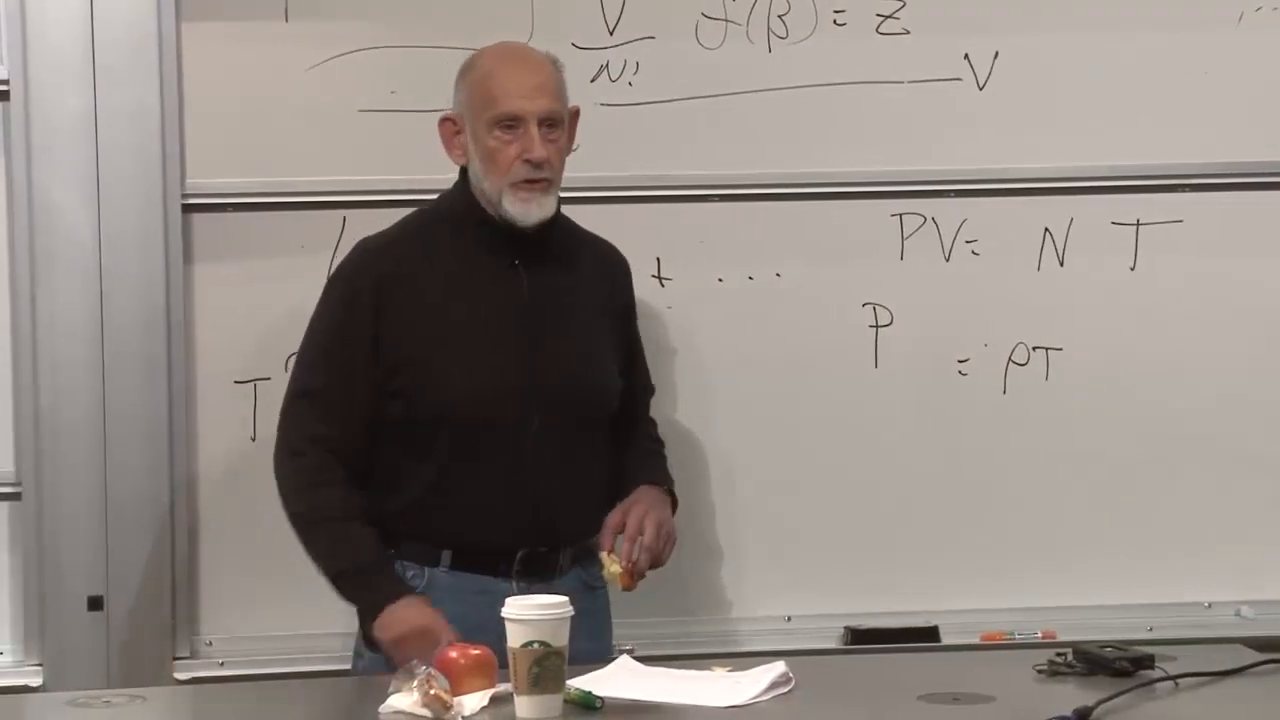
\includegraphics[width=0.90\textwidth]{lecture_05_figure_08.png}
\caption{\(\log Z\)的体积导数以及由此得到的理想气体状态方程\(PV=NT\)，或\(P=\rho T\)。}
\lectureframe{01:09:25}
\end{figure}

恢复实验室温度\(T_K\)，
\begin{equation}
 PV=Nk_BT_K.
 \label{eq:sm5-ideal-gas-law-laboratory}
\end{equation}
这个熟悉的结果与动理学直觉一致，但它的推导现在建立在一个远远超出自由气体的框架之上。

\section{第二个收获：平衡涨落}

压强计算已经完成，但还有一个承诺过的问题：还能从配分函数中提取什么？考虑一个与热浴热接触的系统。它的能量并不固定。能量进入和离开，因此重复测量会在正则平均值附近涨落。

\begin{classroomqa}
\audiencequestion{我们现在能计算之前承诺的涨落吗？}
\lecturerresponse{能。额外的时间允许对同一原理进行第二次演示：\(Z\)的导数编码了可测量的热力学信息。
\lecturetimestamp{01:10:37--01:10:50}}
\end{classroomqa}

\subsection{方差与标准差}

对于随机变量\(x\)，其中\(\langle x\rangle=0\)，分布宽度的一种度量是\(\langle x^2\rangle\)。对于一般分布，将变量平移其均值：
\begin{equation}
 \delta x=x-\langle x\rangle.
 \label{eq:sm5-centered-variable}
\end{equation}
它的均值为零，
\begin{equation}
 \langle\delta x\rangle
 =
 \langle x\rangle-\langle x\rangle=0,
 \label{eq:sm5-centered-mean}
\end{equation}
其均方为
\begin{align}
 (\Delta x)^2
 &\equiv
 \left\langle\left(x-\langle x\rangle\right)^2\right\rangle \notag\\
 &=
 \langle x^2\rangle
 -2\langle x\rangle^2
 +\langle x\rangle^2 \notag\\
 &=
 \langle x^2\rangle-\langle x\rangle^2.
 \label{eq:sm5-variance}
\end{align}
这就是方差。它的正平方根\(\Delta x\)是标准差。

\begin{classroomqa}
\audiencequestion{为什么
\(x-\langle x\rangle\)的平均值恰好为零？}
\lecturerresponse{平均是线性的，而\(\langle x\rangle\)已经是一个数。因此
\(\langle x-\langle x\rangle\rangle
=\langle x\rangle-\langle x\rangle=0\)。
\lecturetimestamp{01:14:02--01:14:22}}
\end{classroomqa}

\begin{classroomqa}
\audiencequestion{平方涨落、方差、均方根宽度和标准差之间有什么区别？}
\lecturerresponse{方差是
\((\Delta x)^2=\langle x^2\rangle-\langle x\rangle^2\)。
标准差是它的平方根，\(\Delta x\)。对于零均值变量，标准差也是它的均方根值。
\lecturetimestamp{01:16:39--01:18:38}}
\end{classroomqa}

\begin{figure}[t]
\centering
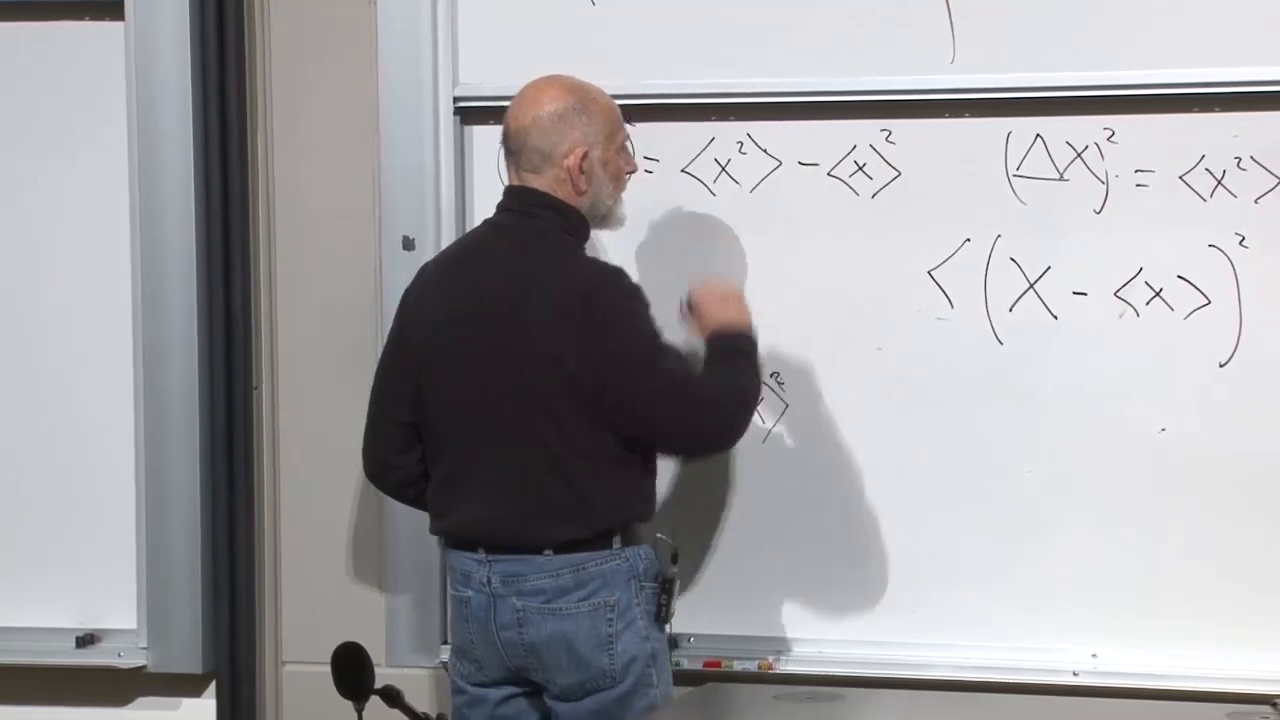
\includegraphics[width=0.90\textwidth]{lecture_05_figure_09.png}
\caption{平移后的变量以及产生\((\Delta x)^2=\langle x^2\rangle-\langle x\rangle^2\)的展开。}
\lectureframe{01:17:20}
\end{figure}

\subsection{由配分函数得到的能量矩}

对于正则系综，
\begin{align}
 \langle E\rangle
 &=
 \frac{1}{Z}\sum_i E_i e^{-\beta E_i} \notag\\
 &=
 -\frac{1}{Z}\frac{\partial Z}{\partial\beta}
 =
 -\frac{\partial\log Z}{\partial\beta}.
 \label{eq:sm5-mean-energy-from-z}
\end{align}
乘以一个\(E_i\)因子由一个负\(\beta\)导数产生。二阶导数生成\(E_i^2\)：
\begin{equation}
 \langle E^2\rangle
 =
 \frac{1}{Z}\sum_i E_i^2e^{-\beta E_i}
 =
 \frac{1}{Z}\frac{\partial^2 Z}{\partial\beta^2}.
 \label{eq:sm5-second-energy-moment}
\end{equation}
因此能量方差为
\begin{align}
 (\Delta E)^2
 &=
 \langle E^2\rangle-\langle E\rangle^2 \notag\\
 &=
 \frac{1}{Z}\frac{\partial^2Z}{\partial\beta^2}
 -
 \frac{1}{Z^2}
 \left(\frac{\partial Z}{\partial\beta}\right)^2 \notag\\
 &=
 \frac{\partial^2\log Z}{\partial\beta^2}
 =
 -\frac{\partial\langle E\rangle}{\partial\beta}.
 \label{eq:sm5-energy-variance-beta}
\end{align}
再一次，一个看起来复杂的可观测量变成了\(\log Z\)的导数。

\begin{figure}[t]
\centering
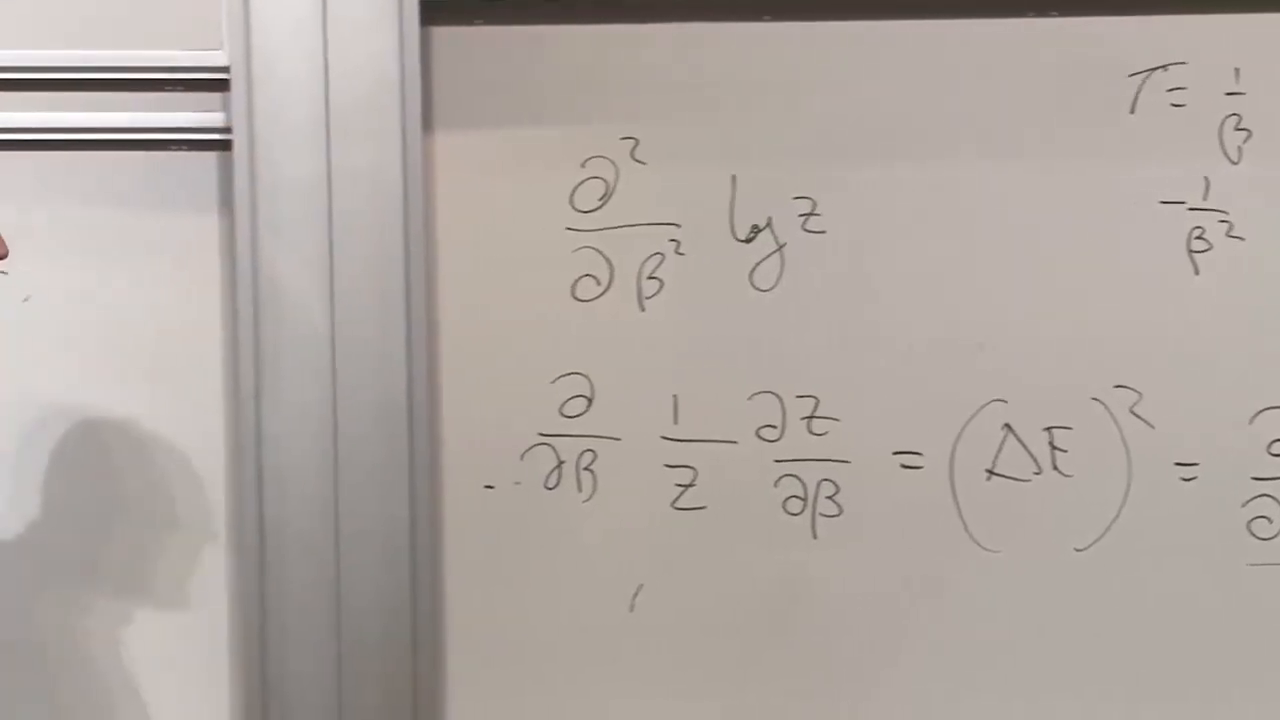
\includegraphics[width=0.90\textwidth]{lecture_05_figure_10.png}
\caption{\(\log Z\)的二阶\(\beta\)导数被等同于能量方差。}
\lectureframe{01:29:00}
\end{figure}

\subsection{热容与涨落的大小}

在讲义单位中\(T=1/\beta\)，所以
\begin{equation}
 -\frac{\partial}{\partial\beta}
 =
 T^2\frac{\partial}{\partial T}.
 \label{eq:sm5-beta-temperature-derivative}
\end{equation}
在固定体积下，定义整个样本的热容为
\begin{equation}
 C_V\equiv
 \left(\frac{\partial\langle E\rangle}{\partial T}\right)_V.
 \label{eq:sm5-heat-capacity}
\end{equation}
方程\eqref{eq:sm5-energy-variance-beta}变为
\begin{equation}
 \boxed{(\Delta E)^2=T^2C_V}
 \qquad (k_B=1).
 \label{eq:sm5-energy-fluctuation-lecture-units}
\end{equation}
对于实验室温度\(T_K\)，其中
\(\beta=(k_BT_K)^{-1}\)，
\begin{equation}
 \boxed{(\Delta E)^2=k_BT_K^2C_V}.
 \label{eq:sm5-energy-fluctuation-laboratory}
\end{equation}

\begin{figure}[t]
\centering
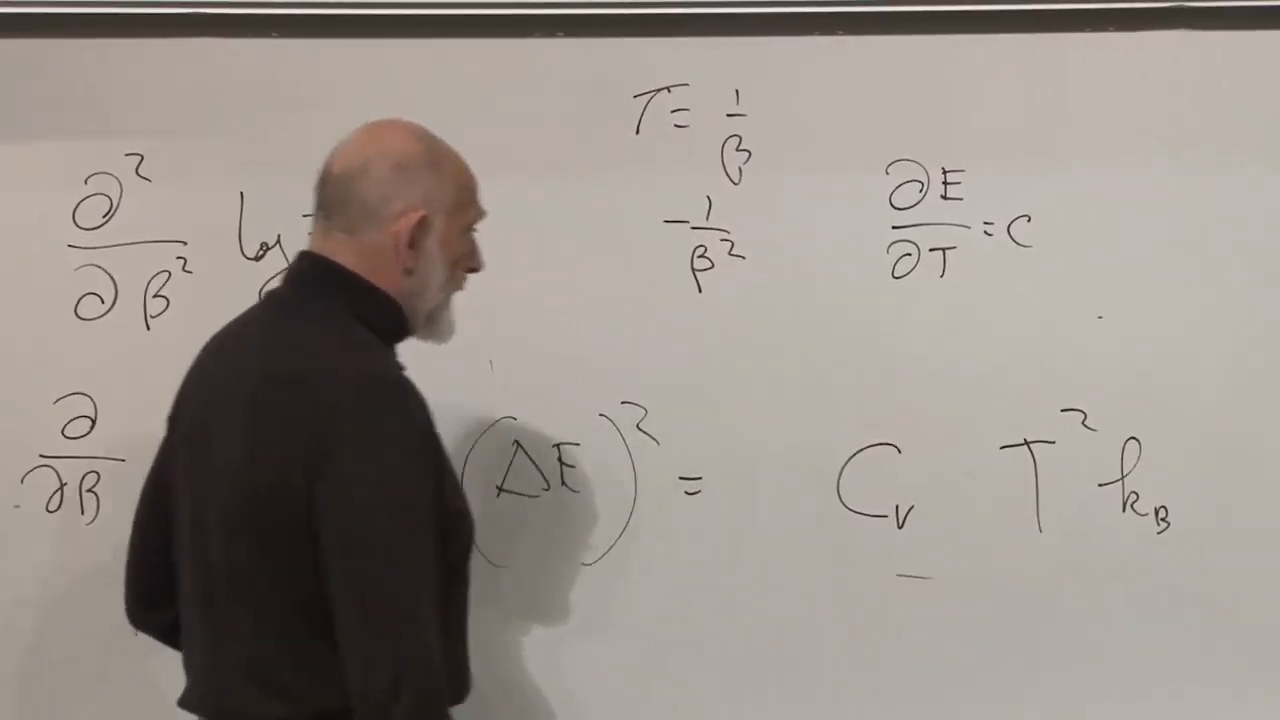
\includegraphics[width=0.90\textwidth]{lecture_05_figure_11.png}
\caption{从\(\beta\)导数到定容热容的转换，其中恢复了\(k_B\)因子。}
\lectureframe{01:31:10}
\end{figure}

\begin{classroomqa}
\audiencequestion{该导数必须指定固定体积而非固定压强吗？}
\lecturerresponse{是的。这一正则推导保持哈密顿量的外部控制参数固定，其中包括\(V\)。所得的量是\(C_V\)。定压系综允许体积和功发生涨落，并需要相应的热力学势；不能简单地在\eqref{eq:sm5-energy-fluctuation-laboratory}中把\(C_V\)替换为\(C_P\)。
\lecturetimestamp{01:29:01--01:29:28; 01:32:50--01:33:21}}
\end{classroomqa}

\begin{classroomqa}
\audiencequestion{\(C_V\)是材料常数吗？}
\lecturerresponse{一般而言不是。它可能依赖于温度、体积、相和组成。此外，这里的\(C_V\)是整个样品的热容，是广延量。只有除以质量、粒子数或物质的量之后，才得到比热。
\lecturetimestamp{01:31:47--01:32:21; 01:33:23--01:34:55}}
\end{classroomqa}

对于普通的广延物质，\(C_V\)正比于\(N\)，因此\((\Delta E)^2\)正比于\(N\)，而\(\Delta E\)正比于\(\sqrt{N}\)。平均能量本身正比于\(N\)。因此
\begin{equation}
 \frac{\Delta E}{\langle E\rangle}\sim\frac{1}{\sqrt{N}}.
 \label{eq:sm5-relative-fluctuation-scaling}
\end{equation}
宏观相对涨落极小，而微观样品则直接显示出这些涨落。\(k_B\)出现在\eqref{eq:sm5-energy-fluctuation-laboratory}中，标志着热力学可观测量与分子离散性之间的这种联系；等价地说，它把宏观单位与阿伏伽德罗尺度的计数联系起来。

压强和涨落现在已从同一个对象中涌现出来：
\[
 P=T\left(\frac{\partial\log Z}{\partial V}\right)_T,
 \qquad
 (\Delta E)^2=\frac{\partial^2\log Z}{\partial\beta^2}.
\]
这就是核心教训。一旦确定了正确的约束，配分函数就不仅仅是对概率进行归一化。它的导数组织起系统可测量的热力学。